\chapter{Algoritmos sustracción del fondo}\label{chap:algoritmos}

\section{Introducción}


Esta capítulo hace una presentación de tres métodos basados en modelos estadísticos para describir el segundo plano de una secuencia y hacer separación de objetos en movimiento de las imágenes del fondo. Se describe el modelo de \textit{Zivkovic y Heidjen} \cite{zivkovic_efficient_2006} de Mixtura de Gaussianas, el cual constituye la base de la mejora propuesta por \textit{Zezhi Chen} \cite{chen_vehicle_2012}, se incluye el trabajo de \textit{Salvadori y Petracca} \cite{salvadori_gaussian_2012} que incorpora el modelo de mixtura de componentes gaussianos (\textit{GMM}) en micro-controladores. Estos modelos son los algoritmos sobre los cuales se desarrolla este trabajo de tesis. También se describe un modelo no-paramétrico (Elgammal et al\cite{elgammal_nonparametricmodel_2000}) para describir el fondo de una imagen. Todos los modelos basado en mixtura de componentes gaussianos han sido incluidos en el desarrollo del sistema de software que permite ejecutar, para luego  comparar y evaluar desempeño sobre las secuencias proporcionadas por MuHAVI, descritos más adelante en el capítulo~\ref{sistema_de_software}. El algoritmo de \textit{Zivkovic y Heidjen} se denomina \textit{MOG} (``\textit{Mixture of Gaussians}'') y el de \textit{Zezhi Chen} \textit{SAGMM} (``\textit{Self-Adaptive Mixture of Gaussians}'') y \textit{UCV} para los algoritmos del trabajo de \textit{Salvadori y Petracca}. 




\section{Modelo General}

La idea general del proceso de sustracción de fondo, es obtener y mantener actualizado (con nuevas imágenes) el modelo de la escena del fondo (\textit{background}) de una secuencia de imágenes, con el propósito de detectar movimientos inusuales, objetos en movimiento, dentro de esta secuencia. Se modela el comportamiento de cada uno de los píxeles de la escena, mediante una función de densidad de probabilidad. El concepto se fundamenta, en la suposición que las imágenes de una escena sin objetos en circulación, tienen un comportamiento regular que puede ser descrito por un modelo estadístico. Un evento podría, por ejemplo, ser detectado identificando las partes de la imagen, que no se ajustan con el modelo que describe el fondo. Un nuevo píxel sólo va a ser considerado parte del fondo, si su valor queda completamente descrito por la función de densidad de probabilidad que es mantenida en el modelo de la imagen de fondo. 


Se utiliza el valor de intensidad de un píxel, en el tiempo (o en el transcurso de una secuencia), para construir una función de densidad de probabilidad, que corresponde al modelo estadístico que describe el comportamiento del píxel. Esta densidad de probabilidad puede ser estimada mediante la construcción de modelos paramétricos o no-paramétricos. El primer tipo de modelo utiliza la combinación lineal de un conjunto de distribuciones Gaussianas, en el que cada componente (Gaussiano) es caracterizado por un grupo de parámetros, que identifica los elementos que emergen durante el avance de las imágenes. El segundo tipo es construido a través de una estimación no-paramétrica de la función de densidad de probabilidad. A diferencia del tipo de modelado paramétrico, que estima un conjunto de parámetros de una función de densidad, el no-parametrico emplea una función '\textit{kernel}' (Normal, Uniforme, Epanechnikov, Gaussiano) para construir la forma del función de densidad de probabilidad.



\begin{figure}[h!]
  \centering
      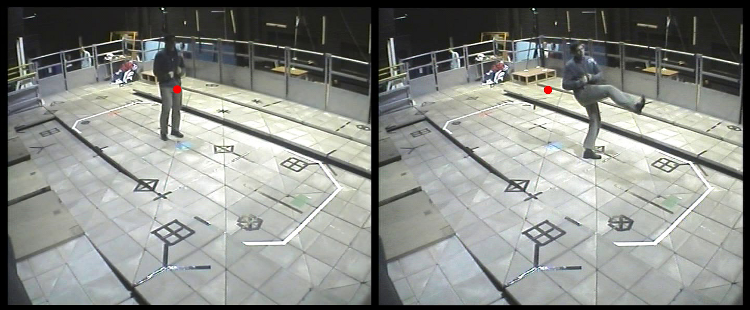
\includegraphics[scale=0.5]{img/ch3/figura_3_1}
  \caption[Imágenes 570, 610 de secuencia ``\textit{Kick Camera 3 Person 4}'']{Imágenes 570 y 610 de la secuencia MuHAVI-MAS ``\textit{Kick Camera 3 Person 4}''. El punto en rojo señala la posición de un píxel en dos eventos diferentes}
\label{posicion_340_160}
\end{figure}

\begin{figure}[h!]
  \centering
      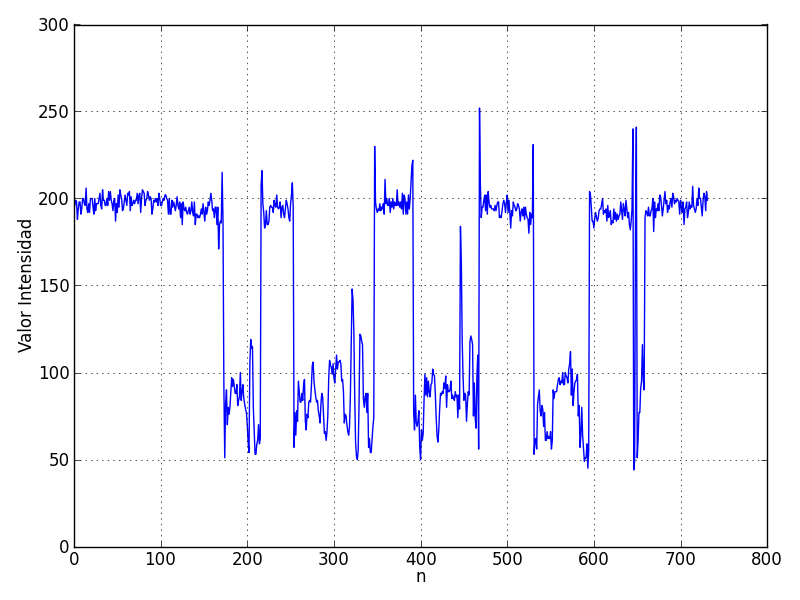
\includegraphics[scale=0.5]{img/ch3/figura_3_2}
  \caption[Cambios de intensidad en el tiempo del valor de un pixel ]{Cambios del valor de intensidad de un color en la secuencia completa.}
\label{intensidad_340_160}
\end{figure}


La separación de píxeles entre elementos del fondo y otros objetos, puede ser explicado en forma simple, mediante las dos imágenes de la figura \ref{posicion_340_160}, tomadas de la secuencia MuHAVI \textit{``Kick Camera 3 Person 4''}\cite{singh_muhavi_2010}. Ambas imágenes señalan el estado de un píxel (punto en rojo) en dos momentos diferentes. El píxel indicado en la imagen de la figura \ref{posicion_340_160}(a), es parte en ese instante del actor (\textit{foreground}), ubicado en medio del escenario, y su valor queda determinado por los colores de su vestimenta. Unos segundos después el actor se encuentra en una posición diferente, realizando una determinada acción. En este nuevo instante el valor del píxel queda definido por los colores del escenario (\textit{background}). La gráfica de la secuencia completa (730 imágenes), que describe el comportamiento del píxel se muestra en la figura \ref{intensidad_340_160}. Los cambios repentinos de intensidad (cambio del nivel 200 al rango de valores 50-100), reflejan los pasos del actor en medio del escenario en la posición donde se encuentra localizado este píxel. Por razones computacionales, se asume que los valores de intensidad de los tres componentes en el espacio RGB (azul, verde y rojo) tienen la misma varianza \cite{zivkovic_efficient_2006}, de esta manera la matriz de covarianza queda definida como una matriz identidad multiplicado por ese único valor de varianza.

\begin{figure}[h!]
  \centering
      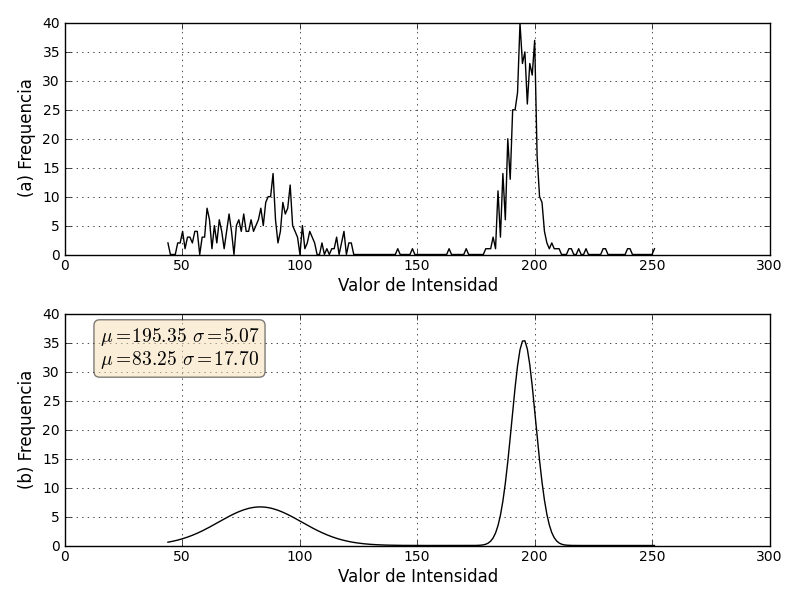
\includegraphics[scale=0.75]{img/ch3/histograma_pixel_340_160_3_2}
  \caption[Histograma secuencia completa ``\textit{Kick Camera 3 Person 4}'']{Histograma secuencia completa ``\textit{Kick Camera 3 Person 4}''}
\label{histograma}
\end{figure}

Al observar el rango valores asociados al escenario en la figura \ref{intensidad_340_160}, se evidencian valores más constantes (o menor dispersión) que los del actor cuando pasa por este píxel. Esto también se puede apreciar en el modelo de la secuencia completa que describe el histograma de la figura ~\ref{histograma}(a). En esta imagen se pueden distinguir dos curvas bien definidas, el fondo de imagen y el el actor en movimiento. La mixtura en este ejemplo, se construye ajustando la función de densidad a dos distribuciones Gaussianas, figura (\ref{histograma})(b). De esta manera, el modelo que describe este píxel en particular para esta secuencia, queda completamente definido por una composición de dos funciones Gaussianas. Se puede ver también en esta figura, que la imagen de fondo puede ser asociada con la componente de menor varianza, debido principalmente a la menor dispersión de valores del fondo. Sin embargo, el menor valor de frecuencia puede ser relacionado con el actor en movimiento, debido al menor tiempo que éste cruza el escenario. 

Se aprovecha estas características de la Mixtura de Gaussianas, para hacer una separación entre \textit{foreground} y \textit{background}. Así cuando la componente Gaussiana que describe algún píxel no se ajuste a la distribución con menor varianza, será considerando parte de un objeto en movimiento. No obstante, si este mismo objeto queda estático por un tiempo considerable, la varianza de su distribución Gaussiana comenzará a disminuir y tomar más relevancia (mayor ponderación relativa) que la varianza del componente del fondo, hasta llegar un momento que será considerado parte del fondo de imagen.




\begin{figure}[h!]
  \centering
      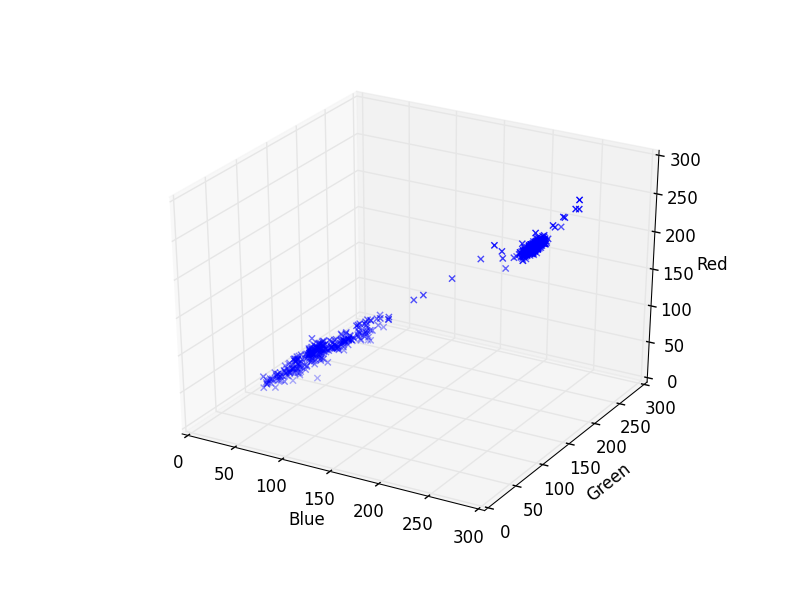
\includegraphics[scale=0.75]{img/ch3/scatter_pt_340_160_3D_Blue_Green_Red}
  \caption[Gráfico dispersión 3D secuencia completa ``\textit{Kick Camera 3 Person 4}'']{Gráfico de dispersión en secuencia ``\textit{Kick Camera 3 Person 4}'' que muestra la nube de puntos relacionados con el escenario y el actor en movimiento.}
\label{scatter_3D}
\end{figure}

\begin{figure}[h!]
  \centering
      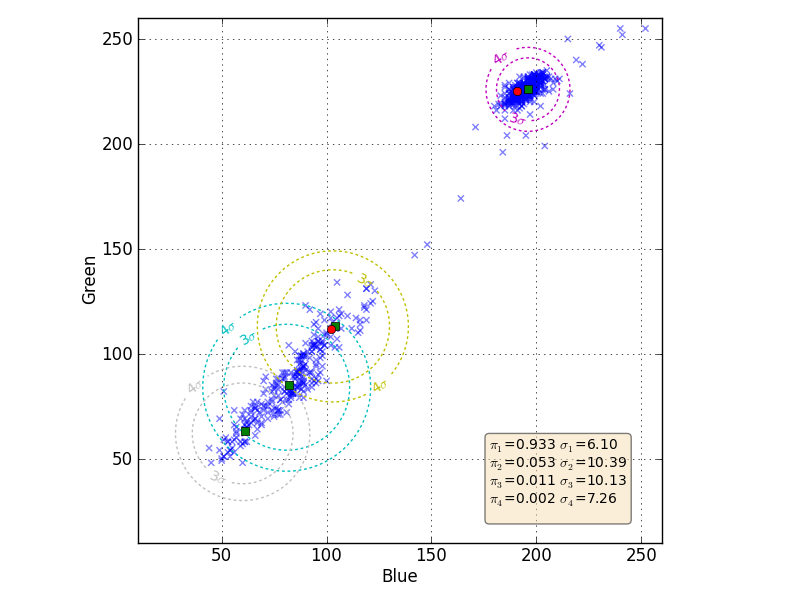
\includegraphics[scale=0.75]{img/ch3/scatter_pt_340_160_isotropic_Blue_Green}
  \caption[Gráfico dispersión 2D secuencia completa ``\textit{Kick Camera 3 Person 4}'']{Gráfico de dispersión secuencia ``\textit{Kick Camera 3 Person 4}'', que muestra dos \textit{cluster} bien definidos}
\label{scatter_2D}
\end{figure}

Los gráficos de las figuras \ref{scatter_3D} y \ref{scatter_2D} sirven de ejemplo para entender el procedimiento de actualización de parámetros, de los diferentes componentes Gaussianos definidos en el algoritmo. Estas figuras son gráficos de dispersión de la secuencia completa (\textit{Kick Camera 3 Person 4}) para el mismo píxel del ejemplo señalado en la figura \ref{posicion_340_160}. La dispersión en la gráfica \ref{scatter_3D}, conforma principalmente dos nubes o \textit{clusters} que se asocian con los dos elementos principales de la secuencia: el escenario y las acciones del actor. El \textit{cluster} más compacto de puntos, localizado en el rango 150-250 de los tres ejes de colores, resume los diferentes tiempos que el píxel fue parte del escenario, mientras el otro \textit{cluster} localizado en la parte inferior refleja la cantidad de veces que el píxel fue parte del actor durante sus movimientos.  

Durante el tiempo que dura la ejecución del algoritmo, los componentes Gaussianos de un píxel van siendo creados o suprimidos en tiempo real, dependiendo exclusivamente de los nuevos valores de entrada y el tiempo de permanencia de estos valores, en alguno de los diferentes \textit{clusters} de la secuencia. Los valores presentan un comportamiento dinámico en directa relación con los eventos de la secuencia; éstos se pueden mover entre \textit{clusters} o bien mantenerse en uno de ellos por un largo periodo. Se aprovecha esta división de \textit{clusters} para hacer la separación entre \textit{background} y \textit{foreground}. La gráfica de la figura \ref{scatter_2D} (dispersión verde-azul) destaca cuatro componentes (\textit{clusters}) definidos por el algoritmo, en el instante que el actor se encuentra detenido de pie en medio del escenario, ejemplo de la figura \ref{posicion_340_160}(a). Los dos puntos en rojo revelan la posición del píxel en los \textit{clusters} para las dos imágenes de ejemplo en la figura \ref{posicion_340_160}. Cada uno de estos componentes tiene un factor de ponderación $\pi_k$ que indica el tiempo de permanencia del píxel en la nube de puntos. Este factor de ponderación es incrementado en la medida que el valor del píxel se mantenga dentro de un margen (de uno de los componentes), determinado por la distancia de Mahalanobis, del punto hacia cada uno de los \textit{clusters}. Para discriminar que el píxel es parte del actor (o el escenario), el algoritmo calcula las distancias del pixel a los ``centroides'' (media) de los diferentes \textit{clusters} establecidos en ese instante. El punto es asociado con algún \textit{cluster}, si el resultado de la distancia de Mahalanobis es menor a tres veces su varianza. Si el punto no es vinculado a ninguno de los clusters definidos en ese momento, el algoritmo crea uno nuevo y deja el punto ligado con este nuevo cluster. Una vez que el algoritmo ha identificado el punto en alguno de los clusters, se realiza la clasificación, ya sea \textit{background}  o \textit{foregorund} y por lo tanto el píxel queda clasificado por la característica del cluster, al que ha sido asociado. Esto es, si el cluster en particular tiene un factor de ponderación más alto que todos los demas, ese cluster es \textit{background} y en consecuencia el píxel también. En caso contrario, el píxel que pertenece a un cluster con factor de ponderación inferior, por lo tanto es algún objeto en movimiento.




\section{Mixtura de distribuciones Gaussianas - GMM}


La superposición de distribuciones Gaussianas que describen el comportamiento de un pixel, se define en la ecuación \eqref{eq:mixturegaussians}. Esta es una sumatoria de \textit{``K''} componentes Gaussianos $\mathcal{N}( x | \mu_k , \Sigma_k)$, cada uno ponderado por un factor multiplicativo $\pi_k$, que establece una función de densidad de probabilidad general para el píxel $p(x)$. El factor de ponderación $\pi_k$, es el grado de influencia de cada componente en el comportamiento global del píxel que esta siendo modelado. Los valores de ponderación pueden ser interpretados, como probabilidades de ocurrencias de las diferentes clases, \textit{Background} y \textit{Foreground}, representadas por los diferentes componentes Gaussianos; por ejemplo, $\pi_1$ podría representar la probabilidad que un píxel sea la imagen de fondo. La suma total de los factores $\pi_k$ es 1, indicado en la ecuación \eqref{eq:mixturefactor}. 

\begin{equation} \label{eq:mixturegaussians}
p(x) = \sum_{k=1}^{K} \pi_k \mathcal{N}( x | \mu_k , \Sigma_k)
\end{equation}

\begin{equation} \label{eq:mixturefactor}
\sum_{k=1}^{K} \pi_k = 1
\end{equation}


Una de las principales tareas del algoritmo que implementa mixtura de Gaussianas, es mantener actualizado los $K$ valores estimados de media ($\mu_1, ..., \mu_k$),  covarianza ($\Sigma_1, ..., \Sigma_k$) y el factor de ponderación ($\pi_1, ..., \pi_k$), por cada píxel de una nueva entrada. Se utilizan los valores de intensidad en el espacio de colores RGB, para construir la mixtura de componentes Gaussianas de un píxel.

La estimación de los parámetros $\vec{\theta} = \{\pi_1,..,\pi_k, \mu_1,..,\mu_k,\Sigma_1,..,\Sigma_k \} $ de las distintas mixturas se realiza mediante el método de Máxima Verosimilitud (\textit{Maximum Likelihood Estimate - MLE}). De esta manera, los parámetros estimados por máxima verosimilitud de un conjunto $t$ de muestras $\mathcal{X} = \{\vec{x}^{(1)}, ..., \vec{x}^{(t)}\}$, quedan determinados por la ecuación (~\ref{eq:maxima_verosimilutd}). Una explicación bien detallada de estimación mediante el método de máxima verosimilitud se puede ver en el capítulo 3 de la referencia \cite{duda_pattern_2000}.

\begin{equation} \label{eq:maxima_verosimilutd}
\hat{\vec{\theta}} = arg \max_{\vec{\theta}}  (\log p(\mathcal{X};\vec{\theta}))
\end{equation}

 
Debido a la dificultad de encontrar una solución analítica de \textit{MLE}, se emplea una aproximación numérica iterativa para maximizar la función de verosimilitud.  El algoritmo de esperanza-maximización (EM) \cite{dempster_maximum_1977}, se usa para encontrar soluciones de máxima verosimilitudes. Este es un procedimiento iterativo que busca un máximo local de la función log-verosimilitud. Este algoritmo es fácil de implementar, sin embargo una de sus limitaciones está en la posibilidad de converger en un máximo local cuando no se ha inicializado.


\subsection{Actualización parámetros del Algoritmo}
\label{subsec:actualizacion_parametros_algoritmo}

Esta parte, describe el método de actualización recursivo que se utiliza en la estimación de los parámetros ($\mu_k$, $\Sigma_k$, $\pi_k$) de cada componente Gaussiano, establecido por \textit{Zivkovic y Heidjen} \cite{zivkovic_efficient_2006}. Por razones computacionales, las matrices de covarianza son consideradas Isotrópicas, es decir la matriz de identidad multiplicado por un único valor de varianza.

El modelo del fondo, es estimado desde un conjunto ``$X$'' de entrenamiento, el cuál mantiene una historia específica de muestras por cada píxel. Para adecuarse a los posibles cambios que puedan producirse, las muestras en este conjunto se actualizan constantemente con nuevas entradas y simultáneamente las más antiguas son eliminadas. Un periodo de adaptación ``$T$'' (100 cuadros) es elegido para mantener la historia más reciente del fondo, y en el instante ``$t$'' se tiene el conjunto de entrenamiento $\mathcal{X_T} = \{x^{(t)}, ..., x^{(t-T)}\}$, desde el cual se estima la función de densidad del fondo.

La parte central del algoritmo, consiste en actualizar constantemente los parámetros $\vec{\theta}$ de las distribuciones Gaussianas, que describen el estado de cada píxel en un momento determinado. Las ecuaciones recursivas para estimar los parámetros de una muestra nueva $x^{(t)}$ en tiempo $t$ se presentan a continuación:


\begin{equation} \label{eq:mixturefactor_update}
\hat{\pi}_k \leftarrow  \hat{\pi}_k + \alpha(o^{(t)}_k - \hat{\pi}_k) - \alpha C_T
\end{equation}
\begin{equation} \label{eq:mixturemu_update}
\hat{\vec{\mu}}_k \leftarrow \hat{\vec{\mu}}_k + o^{(t)}_k (\alpha/\hat{\pi}_k) \vec{\delta}_k
\end{equation}
\begin{equation} \label{eq:mixturesigma_update}
\hat{\sigma}^2_k \leftarrow \hat{\sigma}^2_k + o^{(t)}_k (\alpha/\hat{\pi}_k) (\vec{\delta}^T_k \vec{\delta}_k - \hat{\sigma}^2_k)
\end{equation}
\begin{equation} \label{eq:mahalanobis_distance}
D^{2}_{k}(\vec{x}^{(t)})=\vec{\delta}^T\vec{\delta}_k/\hat{\sigma}^{2}_k
\end{equation}

\[
\vec{\delta}_k = \vec{x}^{(t)} - \hat{\vec{\mu}}_k
\]


El factor constante $\alpha$, define una curva de decaimiento exponencial para limitar la influencia de los datos más antiguos. Se usa esta constante, como reemplazo de $T$ mencionado anteriormente, relacionando ambas constante por la siguiente relación: $\alpha=1/T$. 

El algoritmo mantiene un conjunto dinámico de componentes por cada píxel, esto significa que el número de componentes del modelo es diferente en periodos distintos de la secuencia. Se determina que una nueva muestra es cercana con algunos de los componentes si la distancia de \textit{Mahalanobis} \eqref{eq:mahalanobis_distance} es por ejemplo, menor que tres. Fijando el valor del \textit{ownership} $o^{(t)}_k$ en uno si la muestra es cercana y en cero para el caso contrario. Si la muestra no es cercana a alguno de los componentes ($o^{(t)}_k=0$), se crea uno nuevo con los siguientes valores por defecto $\pi_{k+1} = \alpha$, $\hat{\vec{\mu}}_{k+1}=\vec{x}^{(t)}$ y $\hat{\sigma}_{k+1}=\sigma_0$, con $\sigma_0$ un valor de inicialización de la varianza fijado en el algoritmo.

Este algoritmo representa también los diferentes elementos que surgen en la secuencia, como un conjunto de \textit{clusters} en tiempo real. Un nuevo objeto que ingresa en la secuencia se caracteriza por un \textit{cluster} adicional con un valor de ponderación $\pi_k$ muy inferior a los otros componentes. 

Para determinar el píxel como una imagen de fondo, se ordena los factores de ponderación en forma descendente, y los $B$ \textit{clusters} con mayor ponderación se aproximan al modelo del fondo como se indica en la siguiente ecuación.

\begin{equation} \label{eq:clusters}
B=arg \max_{b}  (\sum_{k=1}^{b} \hat{\pi}_k > (1 - c_f))
\end{equation}

El parámetro $c_f$ es un criterio de medición que indica la cantidad de los datos que pueden ser considerados objetos de \textit{foreground} sin la influencia del modelo de \textit{background}. De esta forma si un nuevo objeto se mantiene estático durante algún tiempo, este será presentado como un \textit{cluster} adicional, y su factor de ponderación $\pi_{k+1}$ será incrementado en la medida que se mantenga estático. Sí se mantiene lo suficiente, y el factor $\pi_{k+1}$ supera $c_f$, entonces este objeto puede ser considerado parte del fondo.


\section{Modelo Mixtura de Gaussianas auto-adaptativo}

Este método se origina en un contexto de vigilancia de tráfico en ciudad. Es el resultado de un sistema de detección y clasificación automática de vehículos \cite{chen_vehicle_2012}, que utiliza una variante del método de mixtura de Gaussianas\cite{zivkovic_efficient_2006}, para hacer una separación entre vehículos en circulación y su pista. La modificación propuesta aborda el problema de cambios bruscos en la iluminación, que podrían transformar todo el segundo plano (\textit{background}) de la imagen, en primer plano (\textit{foreground}). Además, la tasa normal de aprendizaje se transforma en una tasa dinámica en tiempo real. Se intenta con esta modificación, obtener una tasa que se adapte en forma dinámica a los cambios de iluminación. También se utiliza como método de procesamiento previo, un filtro espacial y temporal\cite{chen_background_2009} para compensar las alteraciones producidas por vibraciones de las camaras. Finalmente para afrontar el problema de cambios en iluminación local, como sombras y reflexiones de luz, modifican un algoritmo de extracción de sombras \cite{horprasert_astatistical_1999}, para incorporar el factor de iluminación global.


\subsection{Factor de iluminación global}
En \cite{chen_self-adaptive_2011}, se menciona el modelo de detección de cambio invariante a iluminación (\textit{ICDM}), al proceso que determina el factor de cambio de iluminación global.  Éste es un procedimiento que realiza el cociente uno a uno entre un conjunto ``$s$'' de pixeles de una imagen de entrada ($i_c$) y su imagen de referencia ($i_r$). El factor de iluminación global ``$g$'' se determina como la mediana de todas las divisiones resultantes, ``\textit{Median of Quotient (MofQ)}''.

\begin{equation} \label{eq:mofq}
g = \median_{(s \in S)}  \left(\frac{i_{r,s}}{i_{c,s}}\right)
\end{equation}

Se define además un contador ``$c_k$'' por cada componente Gaussiano en la mixtura. Este contador se utiliza para mantener un registro de cuantos puntos han contribuido en la estimación de parámetros de cada Gaussiana, cada vez que los parámetros de un componente Gaussiano es actualizado, el contador también es incrementado. En caso que un nuevo componente se agrega a la mixtura este contador es inicializado a uno. 

El factor de aprendizaje $\alpha$ es usado como base para construir un nuevo factor de aprendizaje $\beta$, el cual utiliza el contador de componentes Gaussianas mencionado anteriormente. Las nuevas ecuaciones de actualización de parámetros se detallan a continuación:


\begin{equation} \label{eq:sagmm_betha}
\beta_k = \alpha(h + c_k)/c_k
\end{equation}

\begin{equation} \label{eq:sagmm_mu}
\hat{\vec{\mu}}_k \leftarrow \hat{\vec{\mu}}_k + o^{(t)}_k (\beta/\hat{\pi}_k) \vec{\delta}_k
\end{equation}

\begin{equation} \label{eq:sagmm_sigma}
\hat{\sigma}^2_k \leftarrow \hat{\sigma}^2_k + o^{(t)}_k (\beta/\hat{\pi}_k) (\vec{\delta}^T_k \vec{\delta}_k - \hat{\sigma}^2_k)
\end{equation}

\begin{equation} \label{eq:sagmm_ck}
c_k \leftarrow c_k + 1
\end{equation}

\begin{equation} \label{eq:sagmm_delta}
\hat{\vec{\delta}}_k = g \bullet \vec{x}^{t} - \hat{\vec{\mu}}_k
\end{equation}

Si el valor de un pixel de la imagen de fondo varia muy rápidamente, el valor del contador $c_k$ para ese píxel no será muy grande, por lo que el valor de $\beta$ aumentará. Actualizando de esta manera el fondo más rápidamente. Por otra parte si el fondo es muy estable, el valor se $\beta$ se aproximará a $\alpha$. También se observa que la distancia de Mahalanobis es balanceada por el factor de cambio de iluminación global $g$.


\subsection{Filtro espacial y temporal}
Este filtro que prepara la imagen antes de ser procesada por el método modificado de mixturas. Realiza un suavizado de cada componente espectral. En una imagen se habla de dominio espacial para referirse a los píxeles localizados en la matriz de valores y dominio espectral para los componentes de frecuencia obtenidos después de aplicar la transformada de Fourier. El domino espacial se relaciona con el dominio espectral, por medio del teorema de la \textit{convolución}. La convolución (descripción muy básica), es el proceso mover una mascara o kernel píxel a píxel sobre una imagen y obtener un resultado de cada píxel de acuerdo con los coeficientes de la mascara. Los filtros del tipo Gaussiano, tienen la particularidad que en ambos espacios (espacial y espectral) son representados por una función Gaussiana.


\begin{equation} \label{eq:sagmm_filter}
K_{h_s,h_s} = \frac{C}{h_s h_t} k \left( {\| \frac{x^s}{h_s} \|}^2 \right) k \left( {\| \frac{x^t}{h_t} \|}^2 \right)
\end{equation}

$C$ es una constante de normalización, $x^s$ es la parte espacial y $x^t$ la parte temporal, $k(x)$ es un perfil común de kernel (Gaussiano) usado en ambos dominios, temporal y espacial. Las variable $h_s$ y $h_t$ son el ancho de banda de los kernels. 


\begin{figure}[h!]
\centering
\fbox{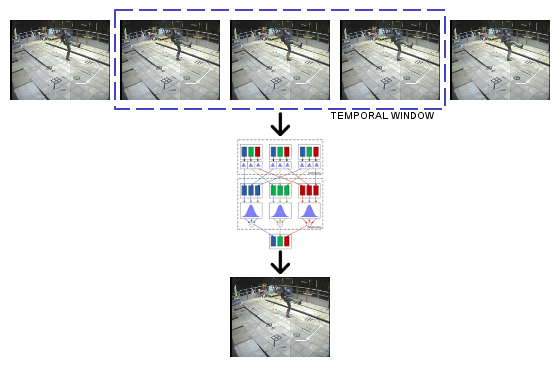
\includegraphics[scale=0.5]{img/ch3/Spatio_Temporal_Filter_Example}}
\caption[Procesamiento temporal de tres imágenes]{Procesamiento temporal de tres imágenes de una secuencia.}
\label{fig:spatio_temporal_filter_example}
\end{figure}


La figura \ref{fig:spatio_temporal_filter_example} es un ejemplo del funcionamiento de este filtro. Se define una ventana temporal que define el número de imágenes que serán procesadas simultáneamente por este filtro. La entrada del filtro, es el número de imágenes que mantiene la ventana temporal, y su salida es la imagen filtrada que será la nueva entrada del algoritmo. Esta ventana puede ser visualizada como un marco que se desliza sobre la secuencia y entrega una imagen procesada como salida.

\begin{figure}[h!]
\centering
%\subfigure{%\documentclass{article}
\documentclass[preview]{standalone}
%\usepackage{tikz}
\usepackage{pgfplots}
%\usepackage{subfigure}

\begin{document}

\newcommand\gauss[2]{1/(#2*sqrt(2*pi))*exp(-((x-#1)^2)/(2*#2^2))} 
\tikzstyle{place}=[circle,draw=blue!50,fill=blue!20,thick]


\begin{tikzpicture}[scale=0.5,cube/.style={very thin,black}]
    %\draw[step=1cm,gray,very thin] (-2,-2) grid (24,24);

    \node[inner sep=0cm] (gaussian) at (2.75,7.5)
        {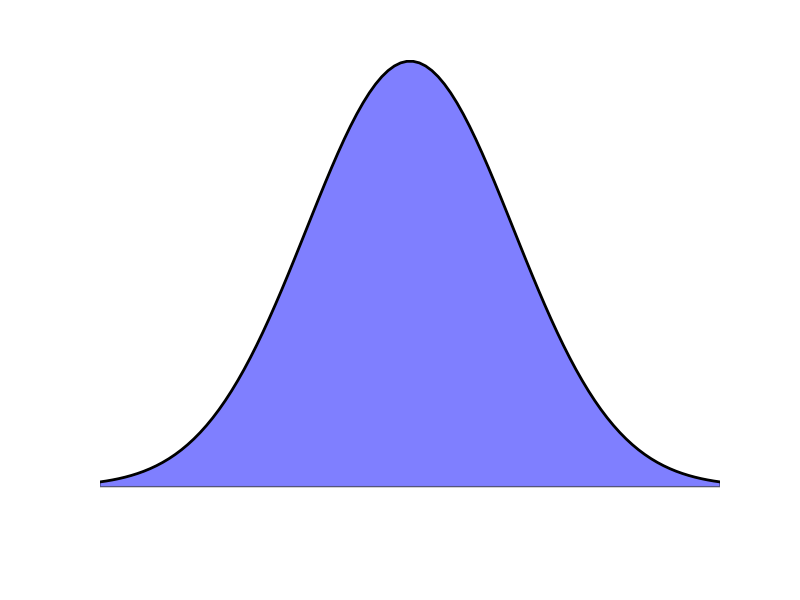
\includegraphics[width=.14\textwidth]{gaussian.png}};
    \node[inner sep=0cm] (gaussian) at (6.75,7.5)
        {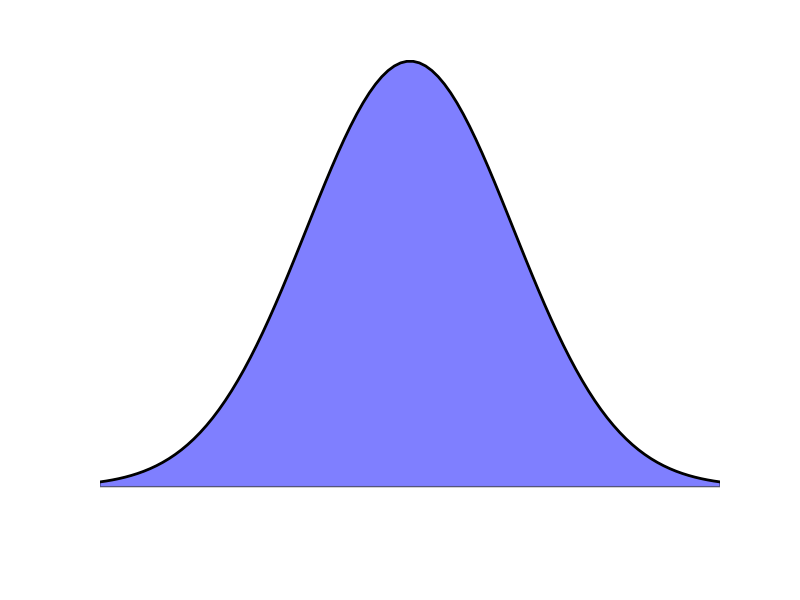
\includegraphics[width=.14\textwidth]{gaussian.png}};
    \node[inner sep=0cm] (gaussian) at (10.75,7.5)
        {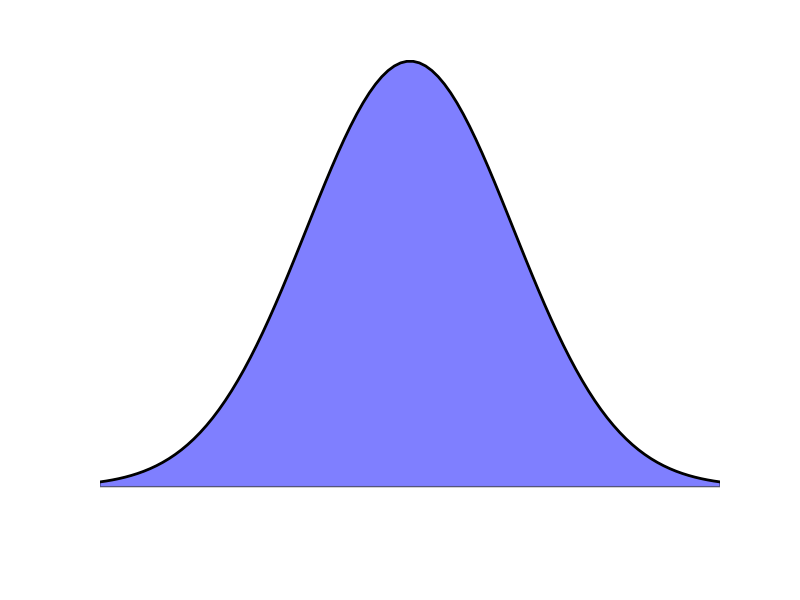
\includegraphics[width=.14\textwidth]{gaussian.png}};

    \node[inner sep=0cm] (gaussian) at (1.5,17.5)
        {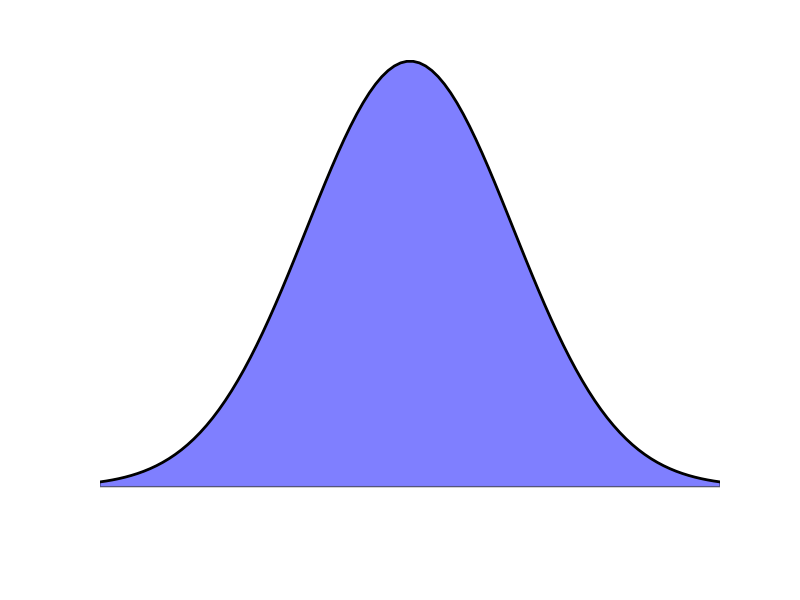
\includegraphics[width=.05\textwidth]{gaussian.png}};
    \node[inner sep=0cm] (gaussian) at (2.5,17.5)
        {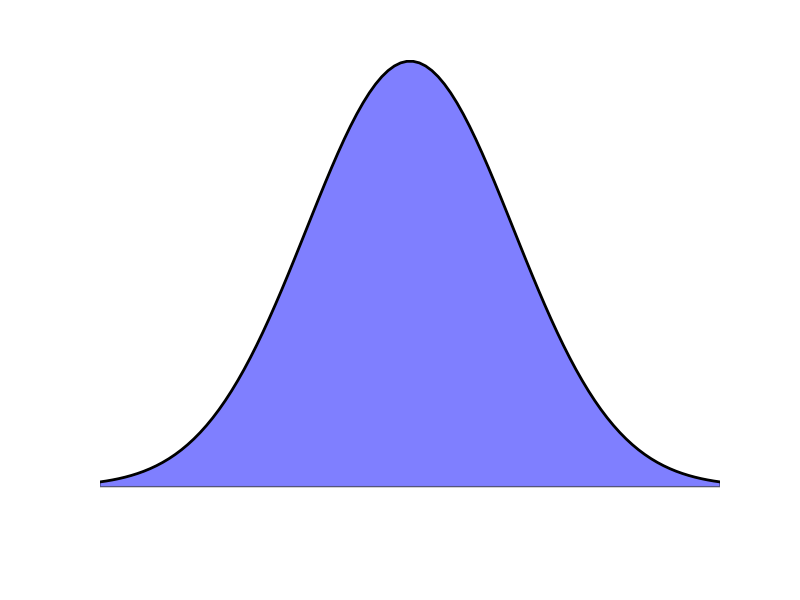
\includegraphics[width=.05\textwidth]{gaussian.png}};
    \node[inner sep=0cm] (gaussian) at (3.5,17.5)
        {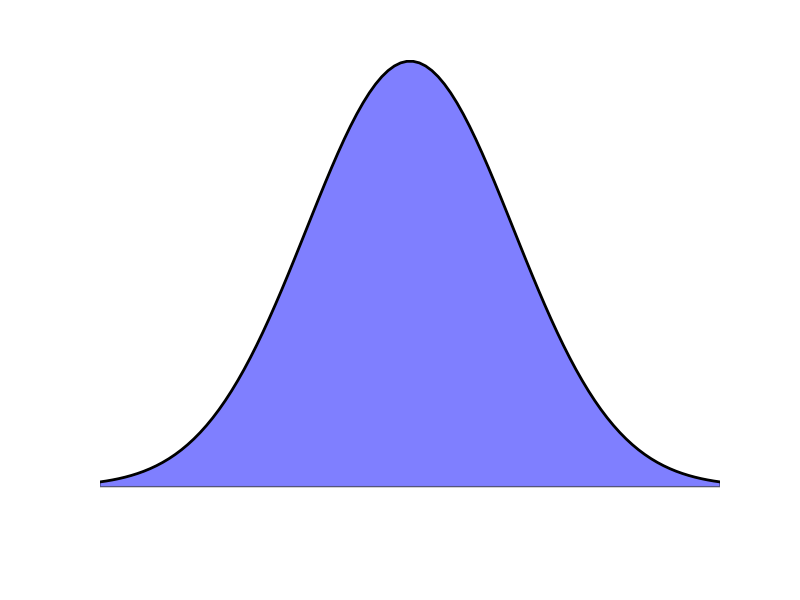
\includegraphics[width=.05\textwidth]{gaussian.png}};

    \node[inner sep=0cm] (gaussian) at (5.5,17.5)
        {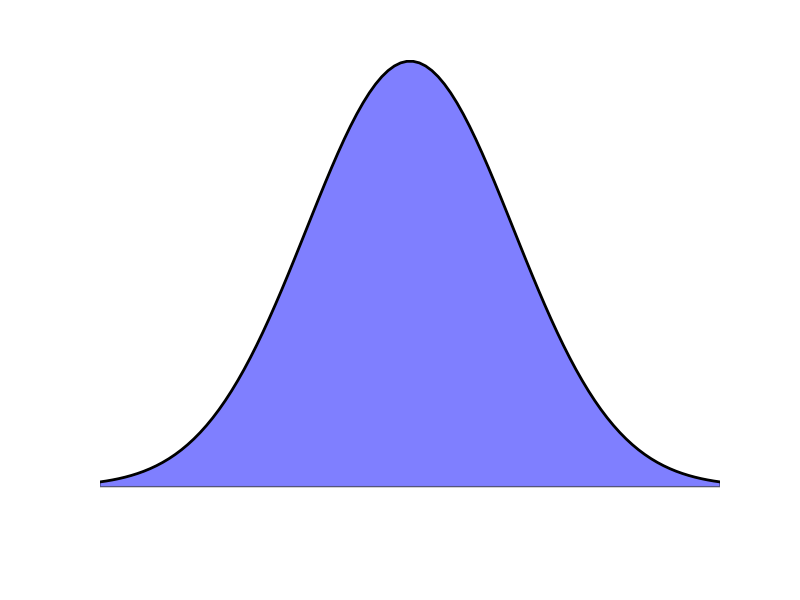
\includegraphics[width=.05\textwidth]{gaussian.png}};
    \node[inner sep=0cm] (gaussian) at (6.5,17.5)
        {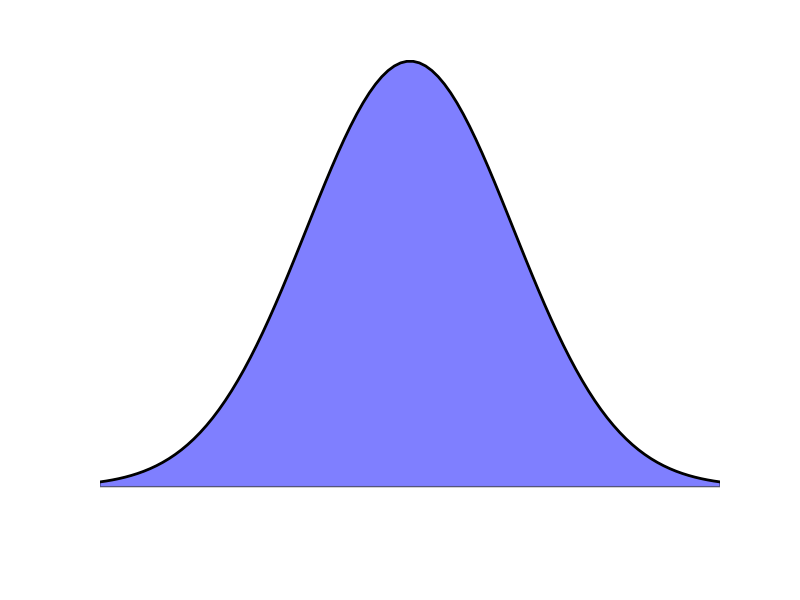
\includegraphics[width=.05\textwidth]{gaussian.png}};
    \node[inner sep=0cm] (gaussian) at (7.5,17.5)
        {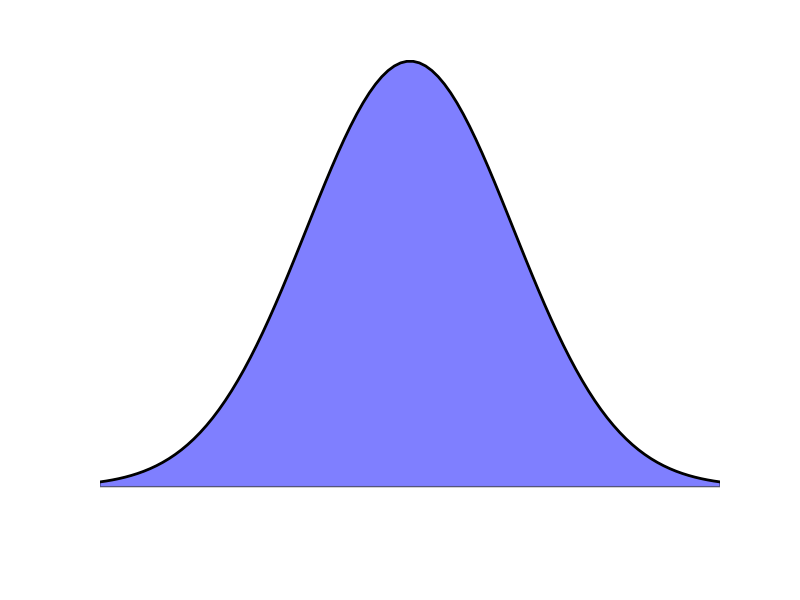
\includegraphics[width=.05\textwidth]{gaussian.png}};

    \node[inner sep=0cm] (gaussian) at (9.5,17.5)
        {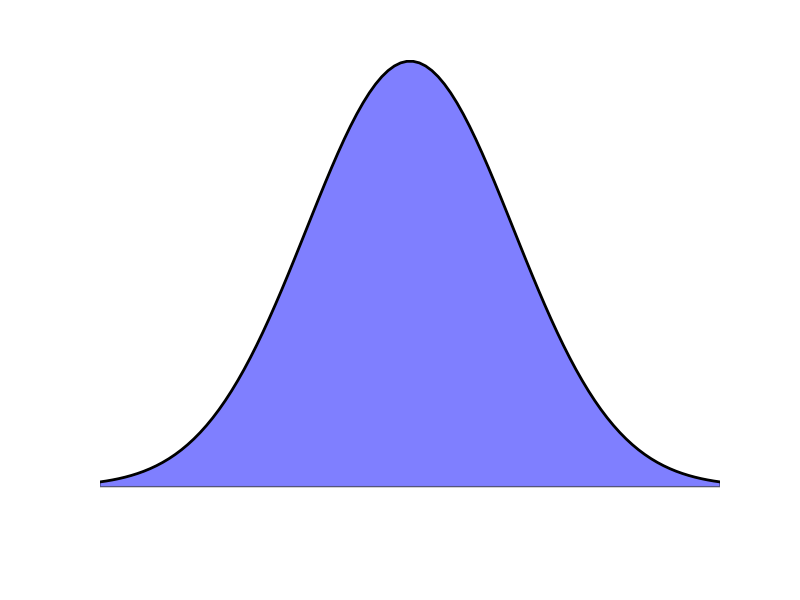
\includegraphics[width=.05\textwidth]{gaussian.png}};
    \node[inner sep=0cm] (gaussian) at (10.5,17.5)
        {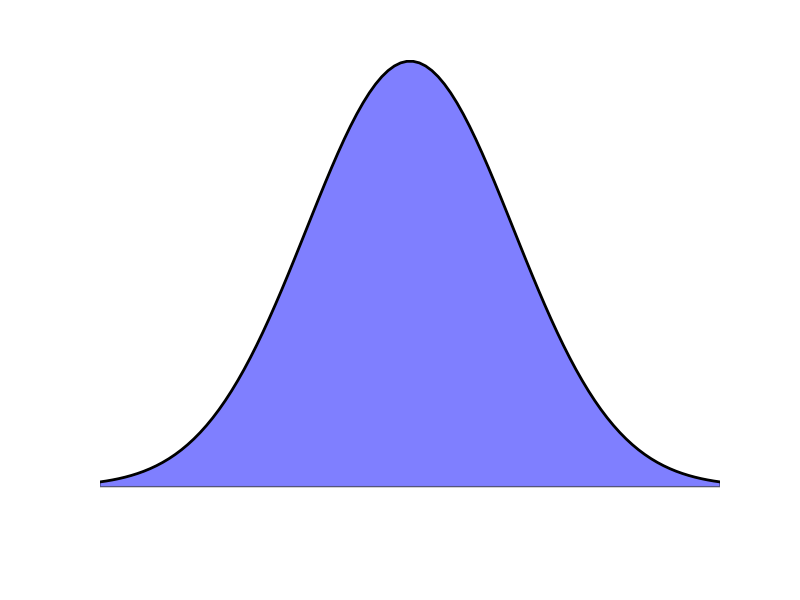
\includegraphics[width=.05\textwidth]{gaussian.png}};
    \node[inner sep=0cm] (gaussian) at (11.5,17.5)
        {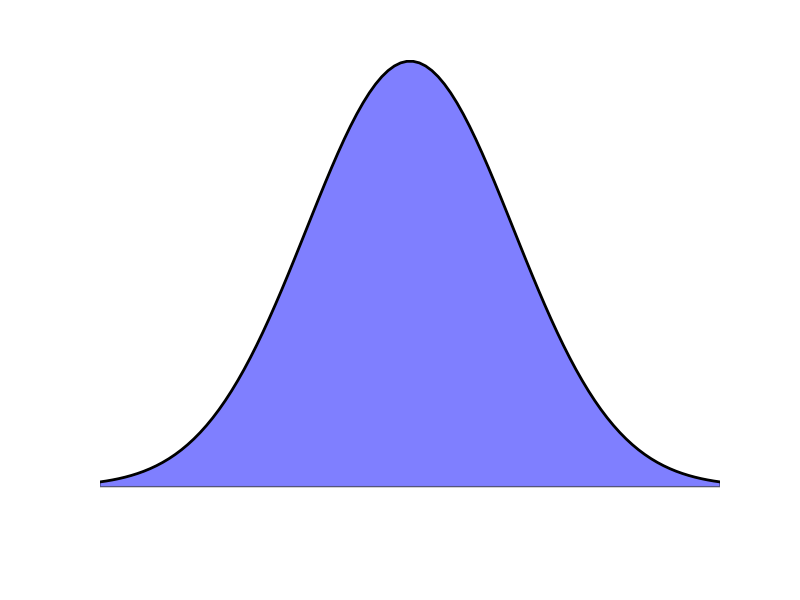
\includegraphics[width=.05\textwidth]{gaussian.png}};

    % First rectangle
    \draw (5,0) rectangle (8.5,3);
    \draw [fill=blue]   (5.5,1) rectangle (6,2);
    \draw [fill=green] (6.5,1) rectangle (7,2);
    \draw [fill=red]     (7.5,1) rectangle (8,2);

    % First gaussian filter
    \draw (1,6) rectangle (4.5,9);
    \draw (5,6) rectangle (8.5,9);
    \draw (9,6) rectangle (12.5,9);

    \draw [->,blue] (1.75,6) -- (2,5);
    \draw [->,blue] (2.75,6) -- (2.75,5.35);
    \draw [->,blue] (3.75,6) -- (3.5,5);
    \draw [->,blue] (2.75,4.5) -- (5,3);

    \draw [->,red] (9.75,6) -- (10,5);
    \draw [->,red] (10.75,6) -- (10.75,5.35);
    \draw [->,red] (11.75,6) -- (11.5,5);
    \draw [->,red] (10.75,4.5) -- (8.5,3);

    \draw [->,green] (5.75,6) -- (6,5);
    \draw [->,green] (6.75,6) -- (6.75,5.35);
    \draw [->,green] (7.75,6) -- (7.5,5);
    \draw [->,green] (6.75,4.5) -- (6.75,3);


    % middle rectangles 
    \draw (1,12) rectangle (4.5,15);
    \draw (5,12) rectangle (8.5,15);
    \draw (9,12) rectangle (12.5,15);

    \draw [fill=blue]   (1.5,13) rectangle (2,14);
    \draw [fill=blue]   (2.5,13) rectangle (3,14);
    \draw [fill=blue]   (3.5,13) rectangle (4,14);

    \draw [fill=green]   (5.5,13) rectangle (6,14);
    \draw [fill=green]   (6.5,13) rectangle (7,14);
    \draw [fill=green]   (7.5,13) rectangle (8,14);

    \draw [fill=red]   (9.5,13) rectangle (10,14);
    \draw [fill=red]   (10.5,13) rectangle (11,14);
    \draw [fill=red]   (11.5,13) rectangle (12,14);

    % small filter rectangles
    \draw (1,17) rectangle (2,18);
    \draw (2,17) rectangle (3,18);
    \draw (3,17) rectangle (4,18);

    \draw (5,17) rectangle (6,18);
    \draw (6,17) rectangle (7,18);
    \draw (7,17) rectangle (8,18);

    \draw (9,17) rectangle (10,18);
    \draw (10,17) rectangle (11,18);
    \draw (11,17) rectangle (12,18);

    % mult. rectangles and nodes
    \node at ( 2.75,10.5) [place] {$(*)$};
    \node at ( 6.75,10.5) [place] {$(*)$};
    \node at ( 10.75,10.5) [place] {$(*)$};

    \node at ( 2.75,19.5) [place] {$(*)$};
    \node at ( 6.75,19.5) [place] {$(*)$};
    \node at ( 10.75,19.5) [place] {$(*)$};

    % arrows of multiple rectangle nodes
    \draw [->,blue] (1.5,17) -- (1.5,15);
    \draw [->,blue] (5.5,17) -- (2.75,15);
    \draw [->,blue] (9.5,17) -- (3.75,15);

    \draw [->,green] (2.5,17) -- (5.5,15);
    \draw [->,green] (6.5,17) -- (6.75,15);
    \draw [->,green] (10.5,17) -- (7.75,15);

    \draw [->,red] (3.5,17) -- (9.5,15);
    \draw [->,red] (7.5,17) -- (10.75,15);
    \draw [->,red] (11.5,17) -- (11.75,15);

    % rectangles
    \draw (1,21) rectangle (4.5,24);
    \draw (5,21) rectangle (8.5,24);
    \draw (9,21) rectangle (12.5,24);

    \draw [fill=blue]   (1.5,22) rectangle (2,23);
    \draw [fill=green]   (2.5,22) rectangle (3,23);
    \draw [fill=red]   (3.5,22) rectangle (4,23);

    \draw [fill=blue]   (5.5,22) rectangle (6,23);
    \draw [fill=green]   (6.5,22) rectangle (7,23);
    \draw [fill=red]   (7.5,22) rectangle (8,23);

    \draw [fill=blue]   (9.5,22) rectangle (10,23);
    \draw [fill=green]   (10.5,22) rectangle (11,23);
    \draw [fill=red]   (11.5,22) rectangle (12,23);


    % sum nodes
    \node at ( 2.75,4.5) [place] {$\sum$};
    \node at ( 6.75,4.5) [place] {$\sum$};
    \node at ( 10.75,4.5) [place] {$\sum$};


\end{tikzpicture}
\end{document}
}
\fbox{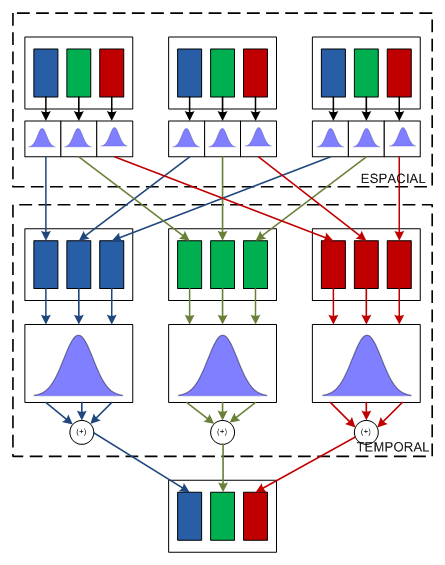
\includegraphics[scale=0.5]{img/ch3/Spatio_Temporal_Filter}}
\caption[Filtro temporal spacial]{Diagrama en bloques del filtro temporal y espacial. La parte de filtro temporal toma tres imágenes y aplica un filtro Gaussiano, el filtro espacial junta los componentes y aplica otro kernel Gaussiano.}
\label{fig:spatio_temporal_filter}
\end{figure}


Una representación en bloques de la implementación de este filtro se puede notar en la figura \ref{fig:spatio_temporal_filter}. La primera etapa es el procesamiento espacial, en que aplica un proceso de difuminado (\textit{blurring}) a cada uno de los colores de una imagen. Este procedimiento, es un suavizado Gaussiano que permite reducir el ruido en la imagen de cada uno de los componentes. La segunda etapa, consiste en agrupar por colores el resultado del filtrado espacial, para luego utilizar un segundo filtro Gaussiano, en cada uno de los tres componentes de las imágenes agrupadas por colores. El resultado es una suma de los tras componentes previamente filtrado. Finalmente, cada uno de los componentes se vuelven a juntar en una sola imagen con tres colores filtrados temporalmente.


La efectividad de este filtro puede ser comparado en los gráficos de la figura \ref{fig:result_spatio_temporal_filter}. La imagen \ref{fig:Figure_A} es el cluster de la imagen de fondo en funcionamiento normal del algoritmo sin filtro aplicado sobre las imágenes. En cambio la imagen de la figura \ref{fig:Figure_B} es el resultado final del cluster de la imagen de fondo,  aplicando procesamiento previo a las imágenes antes de ingresar en el algoritmo. Se puede observar que el cluster final filtrado es mucho más compacto que el otro. Finalmente esta de filtrado es una ayuda en el proceso de separación del fondo de imagen de los elementos móviles.

\begin{figure}[!h]
\centering     %%% not \center
\subfigure[Resultado final sin filtro]{\label{fig:Figure_A}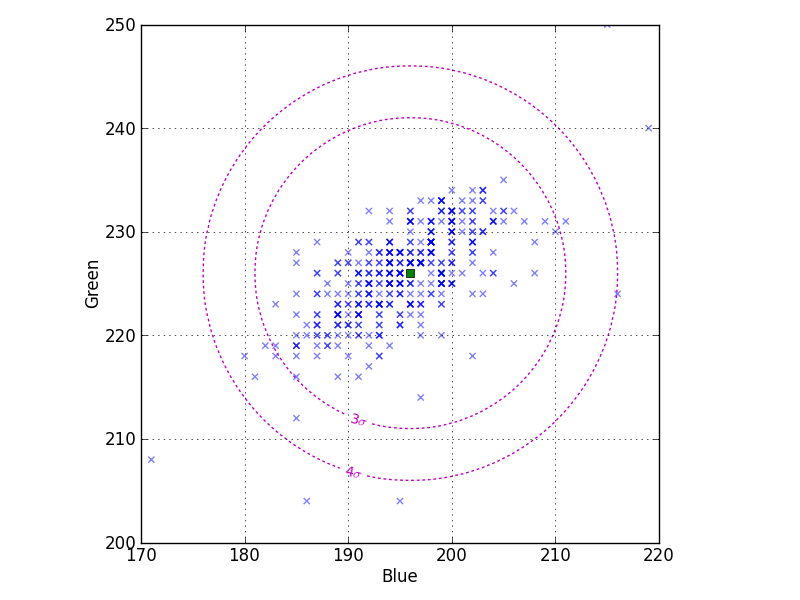
\includegraphics[width=70mm]{img/ch3/cluster_bg_340_160}}
\subfigure[Resultado final con filtro]{\label{fig:Figure_B}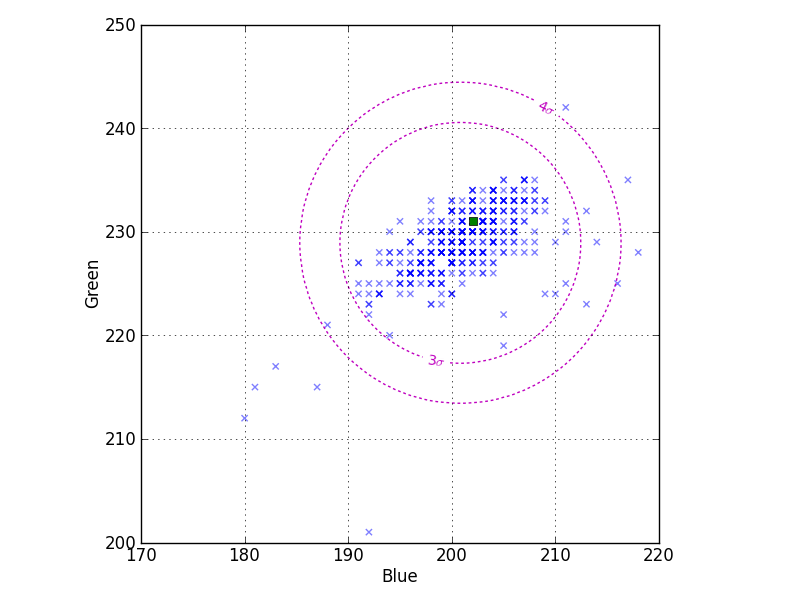
\includegraphics[width=70mm]{img/ch3/cluster_bg_340_160_filter}}
\caption[Comparación de efectividad del filtro en una secuencia completa]{Comparación de efectividad del filtro Espacial-Temporal aplicado en la secuencia completa }
\label{fig:result_spatio_temporal_filter}
\end{figure}

%-----------------------------
\newpage
\section{Modelo GMM incluido en Micro-Controladores}\label{sec:ch3:ucvgmm}
Este método \cite{salvadori_gaussian_2012}, denominado en este trabajo tesis como \textit{UCV}, aborda el problema de incluir el modelo \textit{GMM} en un microcontrolador sin capacidad de procesamiento en punto flotante, en microcontroladores de bajo consumo y bajo costo. En este método, al igual que el original, cada pixel de una imagen de fondo se continua representado por una mixtura de \textit{G} componentes gaussianas, y cada componente por los tres parámetros que describen una gaussiana; media ($\mu$), varianza ($\sigma^2$) y un peso ($w$). Además, se siguen realizando las mismas reglas de actualización definidas previamente en \ref{eq:sagmm_betha}, \ref{eq:sagmm_mu}, \ref{eq:sagmm_sigma}. Sin embargo, estas reglas de actualización son re-definidas mediante una operación de \textit{redondeo}. Se define para esto los conceptos de \textit{granularidad} ($\gamma$), y pasos de actualización \textit{updating step} ($\xi$). 

\begin{equation} \label{eq:ch3:roundfunction}
b=G\_ROUND(a,\xi,\gamma)= \left\{ 
\begin{array}{l l}
\lfloor \frac{a}{\gamma} \rfloor \ast \gamma + \gamma & \quad 
\text{if $(a - \lfloor \frac{a}{\gamma} \rfloor \ast \gamma) \geq \xi$}\\
\lfloor \frac{a}{\gamma} \rfloor \ast \gamma                  & \quad 
\text{if $(a - \lfloor \frac{a}{\gamma} \rfloor \ast \gamma) < \xi$}
\end{array} \right.
\end{equation}

Con \textit{granularidad} $\gamma$ definida desde un conjunto $B=\{ b_i \in N | b_{i+1} - b_i = \gamma\}$, $\xi=\frac{\gamma}{2}$, y $a$ el número a ser redondeado.

\begin{equation}\label{eq:ch3:updating_rule_mu}
\mu_{i+1} = G\_ROUND(\mu_i+k_id_i, \xi_{\mu}, \gamma_{\mu})
\end{equation}
\begin{equation}\label{eq:ch3:updating_rule_sigma}
\sigma^2_{i+1} = G\_ROUND(\sigma^2_i + k_i(D_i-\sigma^2_i), \xi_{\sigma}, \gamma_{\sigma})
\end{equation}

Con $k_i=\frac{\alpha}{w_i}$, $p_i$ valor del de entrada, $d_i=p_i-\mu_i$, y $D_i=d^2_i$

En contraste la regla de actualización de los pesos $w$ de cada componente gaussiano, no depende directamente del valor de entrada del pixel $p_i$, este depende del número de veces (contador $s$) que el pixel $k$ pertenezca a una componente gaussiana $g$. En caso que el pixel no pertenezca a esa componente gaussiana el contador $s$ se decrementa. Se especifica el número de iteraciones necesarias para alcanzar un peso $w$ a través de la siguiente relación:

\begin{equation}\label{eq:ch3:updating_rule_w1}
S(w,\alpha)=\frac{log_{10}(1-w)}{log_{10}(1-\alpha)}
\end{equation}

Con $\alpha$ el factor de aprendizaje. La relación anterior simplifica la actualización de los pesos a una operación de incremento y decremento de un contador. Pero esta relación no puede ser implementada en micro-controladores, por el problema de procesamiento en punto flotante. De esta manera se definen  aproximaciones lineales como solución para obtener el valor del peso $w$ desde un contador de enteros. 

La aproximación lineal (figura \ref{fig:ch3:ucv_weight_linear}) aproxima la relación definida en \ref{eq:ch3:updating_rule_w1} por una recta que pasa por el origen y un punto $P_0=(S(w_0,\alpha), w_0)$ con $w_0=0.5$, y $m=2S(w_0,\alpha)$.


\[
w(s) = \frac{s}{m}
\]


\begin{figure}[!h]
\centering     %%% not \center
\subfigure[Aproximación Lineal]
{\label{fig:ch3:ucv_weight_linear}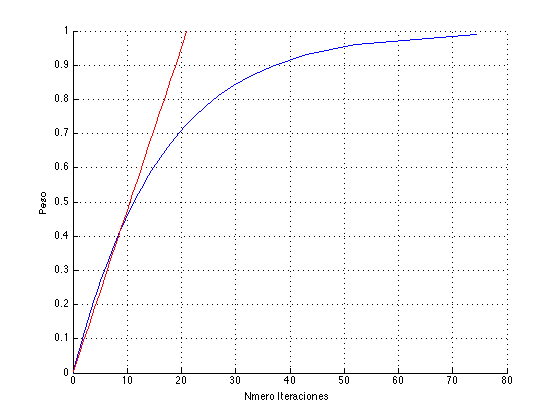
\includegraphics[width=70mm]{img/ch3/ucv_linear}}
\subfigure[Aproximación con dos lineas]
{\label{fig:ch3:ucv_weight_poly}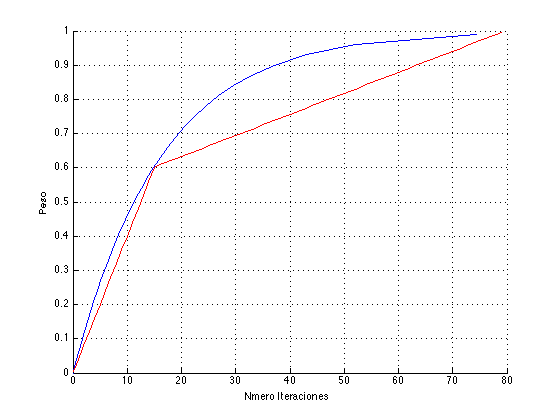
\includegraphics[width=70mm]{img/ch3/ucv_poly}}
\caption[Aproximación de actualización de los pesos]{Aproximación de actualización de los pesos. }
\label{fig:ch3:ucv_weight}
\end{figure}


Las curvas de la figura \ref{fig:ch3:ucv_weight} señalan una simplificación de las reglas de actualización del valor $w$, que determina si una componente Gaussiana pertenece al fondo de la imagen (\textit{Background}) o la silueta (\textit{Foreground}), este valor $w$ es el mismo parámetro $\hat{\pi}_k$ mencionado en la ecuación \ref{eq:mixturemu_update}. Este método aproxima la actualización del parámetro de peso $w$ (\textit{weight}) haciendo aproximación lineal de las curvas logarítmicas como se señala en las curvas de la figura \ref{fig:ch3:ucv_weight}. En el primer caso, aproximación con una recta, la linea recta pasa entre el origen y el punto $w_0=0.5$ y el contador hace un decremento o incremento para lograr el valor de peso requerido. En la segunda figura \ref{fig:ch3:ucv_weight_poly}, un ejemplo de aproximación con dos rectas (puede ser más de dos rectas), cada recta aproxima una componente Gaussiana diferente, una con mayor peso que la otra, la primera curva aproxima a una componente gaussiana de menor peso (\textit{Foreground}), y la segunda de mayor peso (\textit{Background}). La figura \ref{fig:ch3:gmm_bytes} se ilustra una representación (ejemplo tomado desde el trabajo \cite{salvadori_gaussian_2012}) de dos bytes por componente Gaussiano, con la aproximación de una linea (figura \ref{fig:ch3:gmm_linear}) y dos rectas (\ref{fig:ch3:gmm_staircase}).

\begin{figure}[!h]
\centering     %%% not \center
\subfigure[Representación lineal]
{\label{fig:ch3:gmm_linear}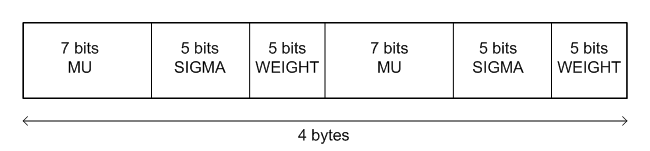
\includegraphics[width=70mm]{img/ch3/gmm_linear}}
\subfigure[Representación con dos lineas]
{\label{fig:ch3:gmm_staircase}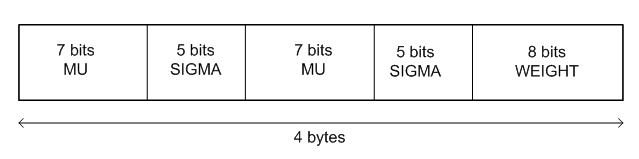
\includegraphics[width=70mm]{img/ch3/gmm_staircase}}
\caption[Representación contadores en 4 bytes]{Representación de contadores en 4 bytes. }
\label{fig:ch3:gmm_bytes}
\end{figure}



%-----------------------------------
\section{Modelo No-Paramétrico de fondo de imagen}
\label{sec:modelo_noparametrico}

%propone obtener la información reciente de una secuencia de imágenes, y actualizar continuamente el modelo del fondo, con la finalidad de capturar cambios repentinos producidos en una escena. Se 
El modelo no-paramétrico de Elgammal et al\cite{elgammal_nonparametricmodel_2000}, plantea que cambios muy bruscos del valor de intensidad de un pixel, en periodos muy cortos de tiempo, no es modelado apropiadamente por un pequeño conjunto de distribuciones Gaussianas, resultando un modelo del fondo no muy preciso. Se demuestra que la distribución de intensidad, para una imagen con cambios significativos es del tipo multimodal. Este método propone obtener solamente la información más reciente de una secuencia de imágenes, y actualizar continuamente el modelo del fondo, de esta manera capturar cambios repentinos producidos en una escena.

En aplicaciones de vigilancia exterior, una escena de fondo que se quiera modelar contiene varios elementos no estáticos, como arbustos o ramas de árboles que se mueven con el viento. Estos elementos producen cambios considerables en los valores de intensidad de un pixel. Se genera en consecuencia un modelo de distribución muy ancho, que abarca un amplio espectro de escala de grises, resultando una detección muy pobre, debido que los colores de los elementos móviles se confunden con los colores contenidos en la imagen de fondo. 

Cada píxel en el modelo del fondo se representa por una función de densidad de probabilidad $P_r(x_t)$ obtenida de $x_1, x_2, ..., x_N$ muestras recientes  de los valores de un píxel. La probabilidad que el valor de un pixel sea $x_t$ en el tiempo $t$ será estimado de manera no-paramétrica utilizando un estimador kernel $K$, como se indica en la siguiente relación. 

\begin{equation} \label{eq:nonparametric}
P_r{(x_t)} = \frac{1}{n} \sum_{i=1}^{N} K(x_t-x_i)
\end{equation}

En esta ecuación $x_t$ es una muestra de un pixel en una imagen nueva que requiere ser clasificado y $K$ es una función kernel del tipo Normal $\mathcal{N}(x | \mu , \Sigma)$, $\Sigma$ representa el ancho de banda de la función de kernel. Se asume que existe independencia entre los distintos canales de colores, por ende $\Sigma$ es una matriz escalar y todos los colores tienen la misma varianza, como se explica en el punto  ~\ref{subsec:actualizacion_parametros_algoritmo}, de esta manera la estimación de densidad se reduce a la siguiente ecuación


\begin{equation} \label{eq:kernel_estimation}
P_r{(x_t)} = \frac{1}{n} \sum_{i=1}^{N} \prod_{j=1}^{d} \frac{1}{\sqrt{2\pi\sigma_{j}^{2}}} e^{-\frac{1}{2}\frac{(x_{t_j}-x{i_j})^2}{\sigma_{j}^{2}}}
\end{equation}

Una vez que la densidad de probabilidad ha sido estimada, el píxel $x_t$ es clasificado como imagen de fondo (\textit{background}) u objeto en movimiento (\textit{foreground}) si la el valor estimado de la densidad está arriba o abajo de cierto valor de umbral. Se usa entonces, esta estimación densidad de probabilidad para considerar un pixel como un elemento móvil, sí $P_r{x_t} < th$. La variable $th$ es un valor global de umbral que puede ser ajustado para lograr un porcentaje específico de falsos positivos. 

Existen dos fuentes de variaciones en el valor de intensidad de un pixel, una es debido a estos cambios bruscos de intensidad, que se proyectan en el pixel en diferentes tiempos y variaciones locales de intensidad debido a un efecto borroso (blurring). El ancho de banda de la función kernel ($\sigma$) refleja estas variaciones locales de intensidad en la imagen y en el tiempo. La varianza local de cada uno de los canales de colores es calculada como la mediana de la diferencia ($x_1-x_{i+1}$) dos pares consecutivos del total de la muestra, independiente para canal de color.

\begin{equation}\label{eq:median}
\sigma = \frac{m}{0.68\sqrt{2}}
\end{equation}


Este método desarrolla además, una segunda de etapa que contribuye en la eliminación de falsos positivos no detectados en la primera etapa del proceso de sustracción de fondo. Estos falsos positivos (denominados falsas detecciones en el trabajo de Elgammal \cite{elgammal_nonparametricmodel_2000}) corresponden por una parte, a ruido aleatorio homogéneo presente en toda una imagen y por otra parte, movimientos que no están representados en el modelo de fondo, como desplazamiento de cámaras o movimientos de ramas de árboles, ambos producidos por la fuerza de viento. Se asume que estos desplazamientos son pequeños entre cuadros de imágenes consecutivos, de esta manera, esto permitiría decidir si un píxel detectado es un elemento del fondo que ha sido movido en una pequeña zona de la región detectada. Se definen dos tipos de probabilidades, la probabilidad de desplazamiento de un pixel $P_N{(x_t)}$, y la probabilidad de desplazamiento de un componente $P_c$. $P_N$ corresponde a la máxima probabilidad del valor de un píxel $x_t$ pertenece a la distribución del fondo en algún punto de la región $N(x)$. 

\begin{equation}\label{eq:displacement_probability}
P_N{(x_t)} = \max_{y \in N(x)} P_r(x_t | B_y)
\end{equation}

\begin{equation}
P_c = \prod_{x \in C} P_N{(x)}
\end{equation}

La probabilidad de desplazamiento de componente $P_c$ se emplea para evitar de detecciones reales sean eliminadas por la primera restricción, se emplea para asegurar que un elemento móvil (\textit{foreground}) se ha desplazado en una zona cercana y no sólo algunos pixeles. Si este componente conectado se desplazado desde la escena del fondo, su probabilidad sería muy baja. Un pixel será, de esta forma, considerado parte de la escena de fondo si cumple con $(P_N(x) > th_1) \wedge (P_C(x) > th_2)$.


Existen dos mecanismos para actualizar el modelo de fondo, con cada nueva muestra de un pixel. En ambos casos cada vez que se agrega una nueva muestra, la muestra más antigua se elimina del conjunto de muestras, para asegurar que la estimación de densidad de probabilidad se base en muestras recientes

\begin{itemize}
\item Actualización selectiva: Se agrega una nueva muestra al modelo únicamente si la muestra es un píxel de la imagen de fondo.
\item Actualización a ciegas: Una nueva muestra se agrega al modelo, independiente si pertenece o no pertenece a la imagen de fondo.
\end{itemize}

 Junto con estos mecanismos de actualización, el modelo de Elgammal et al\cite{elgammal_nonparametricmodel_2000} mantiene además, dos modelos de fondos: largo y corto plazo 

\begin{itemize}
\item Modelo de corto plazo, es un modelo reciente de la escena que utiliza las primeras $N$ muestras, utilizando actualización selectiva.
\item Modelo de largo plazo, es un modelo que emplea un número mayor de muestras (el total de la ventana de muestras) y por lo tanto contiene una versión más estable de la escena. Las muestras de este modelo se actualizan utilizando el mecanismo de actualización a ciegas.
\end{itemize}

\section{Resumen}

En este capítulo se ha hecho una revisión detallada de los principales algoritmos basados en mixtura de componentes gaussianas (\textit{GMM}). La idea principal de estos algoritmos consiste en modelar el valor de intensidad de un pixel (o un grupo en el espacio de colores RGB) y construir una función de densidad en el transcurso del tiempo, la densidad se puede estimar mediante una mixtura de componentes Gaussianas. Se discrimina si un pixel pertenece a un objeto en movimiento o la imagen de fondo, verificando el comportamiento de las varianzas de las componentes Gaussianas. Se ha descrito principalmente el modelo de el modelo de Zivkovic\cite{zivkovic_recursive_2004} y Chen\cite{chen_vehicle_2012}. El próximo capítulo tratará de las principales métricas de evaluación de desempeño, se hará una descripción de los diferentes métodos de evaluación y las métricas que sirven para esos métodos.